\section{Background and Problem}

\begin{frame}
	\frametitle{Planning under Uncertainty}
	\framesubtitle{Domain Characteristics}
	
	\begin{columns}[T]
		\begin{column}{.7\textwidth}
			\begin{itemize}
				\item A system is controlled by one or more \textit{agents}
				\item \textit{Uncertain domain dynamics}, i.e.\\ uncertainty may be present in:
				\begin{itemize}
					\item Execution of actions (e.g., robot may slip)
					\item Exogenous factors (e.g., doors open/closed)
					\item Percepts (e.g., sensor noise)
				\end{itemize}
				\item \textit{Sequential decision making}
				\begin{itemize}
					\item Non-myopic agents
					\item Selection of actions with high future pay-off
				\end{itemize}
			\end{itemize}
		\end{column}
		\begin{column}{.35\textwidth}
		%	%\vspace{-30pt}
			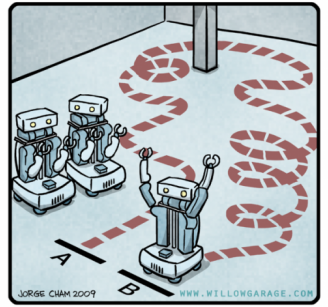
\includegraphics[width=1.0\textwidth, right]{figures/path-planning2}
		\end{column}
	\end{columns}
\end{frame}

\begin{frame}
	\frametitle{Planning under Uncertainty}
	\framesubtitle{Example Domains}
	
	\begin{columns}[t]
		\begin{column}{.3\textwidth}
			\centering 
			\begin{overlayarea}{\linewidth}{4.75cm}
				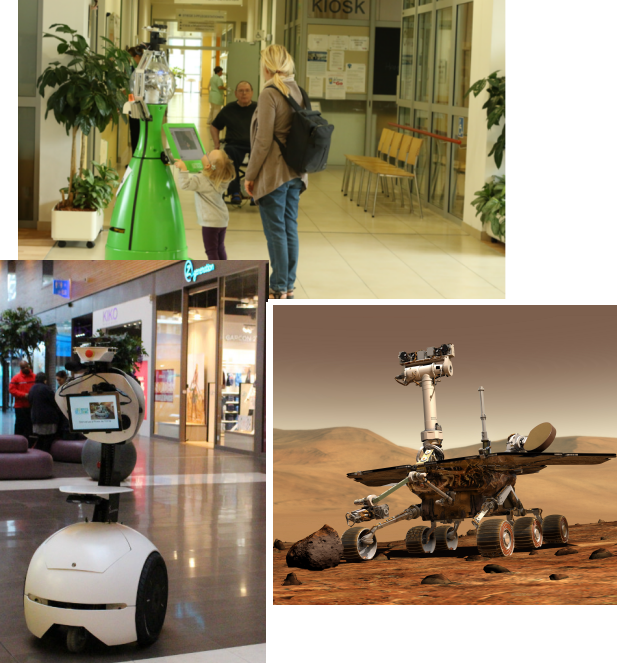
\includegraphics[width=\columnwidth]{figures/path-planning}
			\end{overlayarea}
			\captionof*{figure}{\scriptsize\textit{\textcolor{tudBlack}{Path planning}}}
		\end{column}
		\begin{column}{.25\textwidth}
			\centering
			\begin{overlayarea}{\linewidth}{4.75cm}
				\centering
				\vspace{-18pt}
				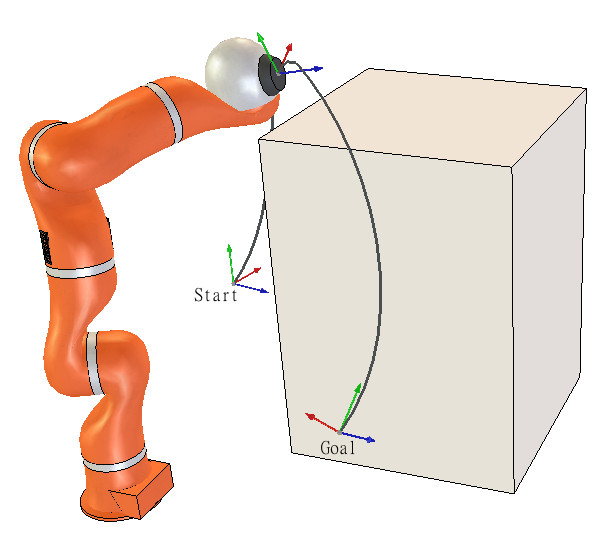
\includegraphics[width=0.75\columnwidth]{figures/motion-planning}\\
				{\scriptsize\textit{Motion planning}}\\\vspace{6pt}
				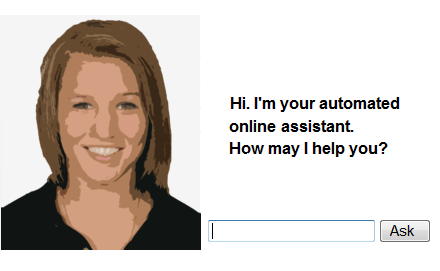
\includegraphics[width=0.85\columnwidth]{figures/dialog_system_2}
			\end{overlayarea}
			\captionof*{figure}{\scriptsize\textit{\textcolor{tudBlack}{Dialog Management}}}
		\end{column}
		\begin{column}{.3\textwidth}
			\centering
			\begin{overlayarea}{\linewidth}{4.75cm}
				\vspace{0pt}
				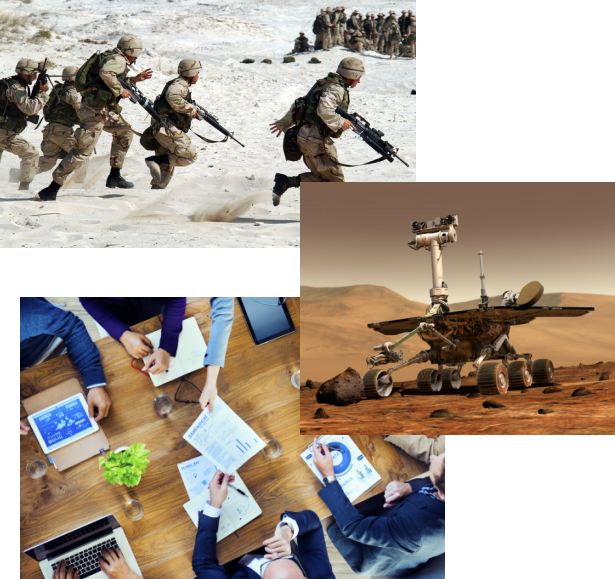
\includegraphics[width=\columnwidth]{figures/operations-planning5}
			\end{overlayarea}
			\captionof*{figure}{\scriptsize\textit{\textcolor{tudBlack}{Operations planning}}}
		\end{column}
	\end{columns}
	\imgsrc*[Image credits]{Hawes et al. \cite{hawes2016strands}, \href{https://coaches.greyc.fr}{Iocchi et al.} \cite{iocchi2016practical}, \href{http://www.coppeliarobotics.com/helpFiles/en/motionPlanningModule.htm}{V-REP Manual}, Bemidji State University}
\end{frame}
% Examples Operations Planning:
% - Military Operations Planning: Decision-Theoretic Military Operations Planning
% - Markov Decision Processes in AI: (Operations Planning Rover Exploration) https://www.safaribooksonline.com/library/view/markov-decision-processes/9781118620106/xhtml/Chapter15.html
% - Project Management: Engineering the Decision-Making Process Using Multiple Markov Theories and DEMO
\imgsrc*{off}

\begin{frame}
	\frametitle{Planning under Uncertainty}
	\framesubtitle{Typical Development Routine}
	\centering
	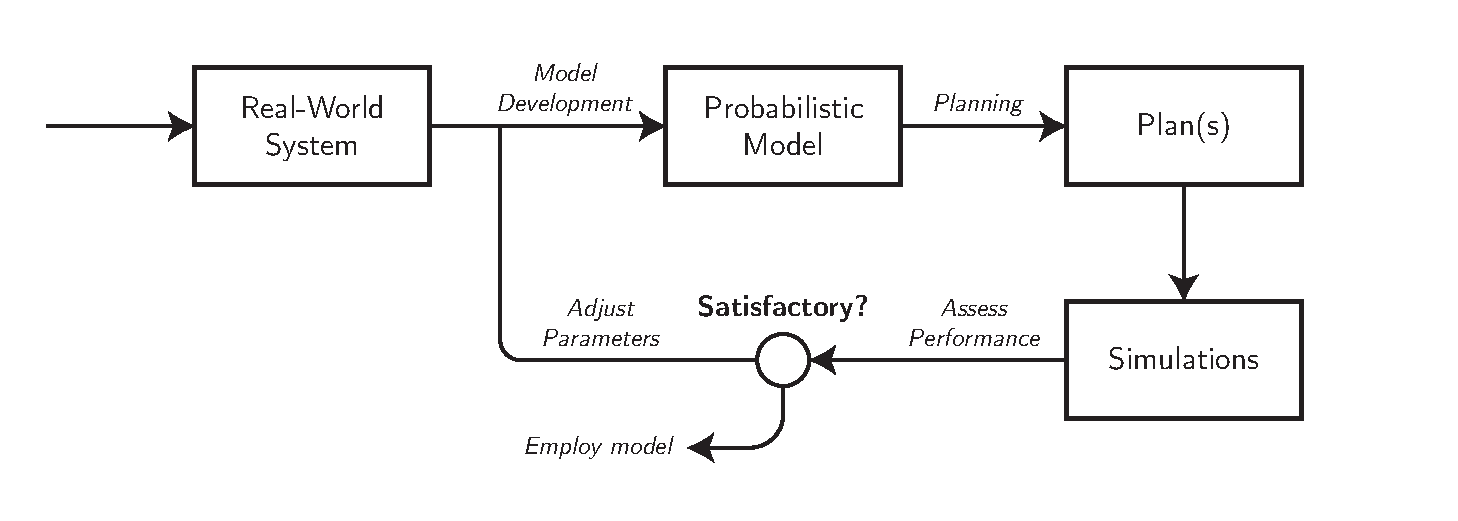
\includegraphics[width=\textwidth]{figures/high-level-planning-diagram}
\end{frame}

\begin{frame}
	\frametitle{Planning under Uncertainty}
	\framesubtitle{Markov Decision Processes (MDPs)}
	
	In DTP systems are modeled by probabilistic models, e.g. MDPs:
	\begin{columns}[T]
		\begin{column}{0.6\textwidth}
			\begin{definition}
				An MDP is a 5-tuple $\mathcal{M} = (\mathcal{S}, s_0, A, \delta, R)$:
				\begin{itemize}
					\item $\mathcal{S}$ is the state-space, $s_0 \in \mathcal{S}$ the initial state
					\item $A$ is the action-space
					\item $\delta: \mathcal{S} \times A \times \mathcal{S} \mapsto [0, 1]$ is the transition function % $\delta: S \times S \times A \mapsto [0,1]$
					\item $R: \mathcal{S} \times A \times \mathcal{S} \mapsto \mathbb{R}$ is the reward function
				\end{itemize}
			\end{definition}
		\end{column}
		\begin{column}{0.425\textwidth}
			\vspace{26pt}
			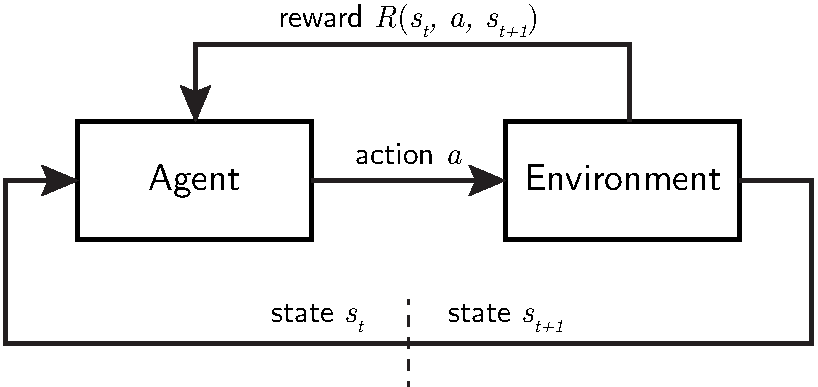
\includegraphics[width=\linewidth]{figures/mdp-2v2}
		\end{column}
	\end{columns}
\end{frame}

\begin{frame}
	\frametitle{Planning under Uncertainty}
	\framesubtitle{Planning with MDPs}
	\begin{center}
	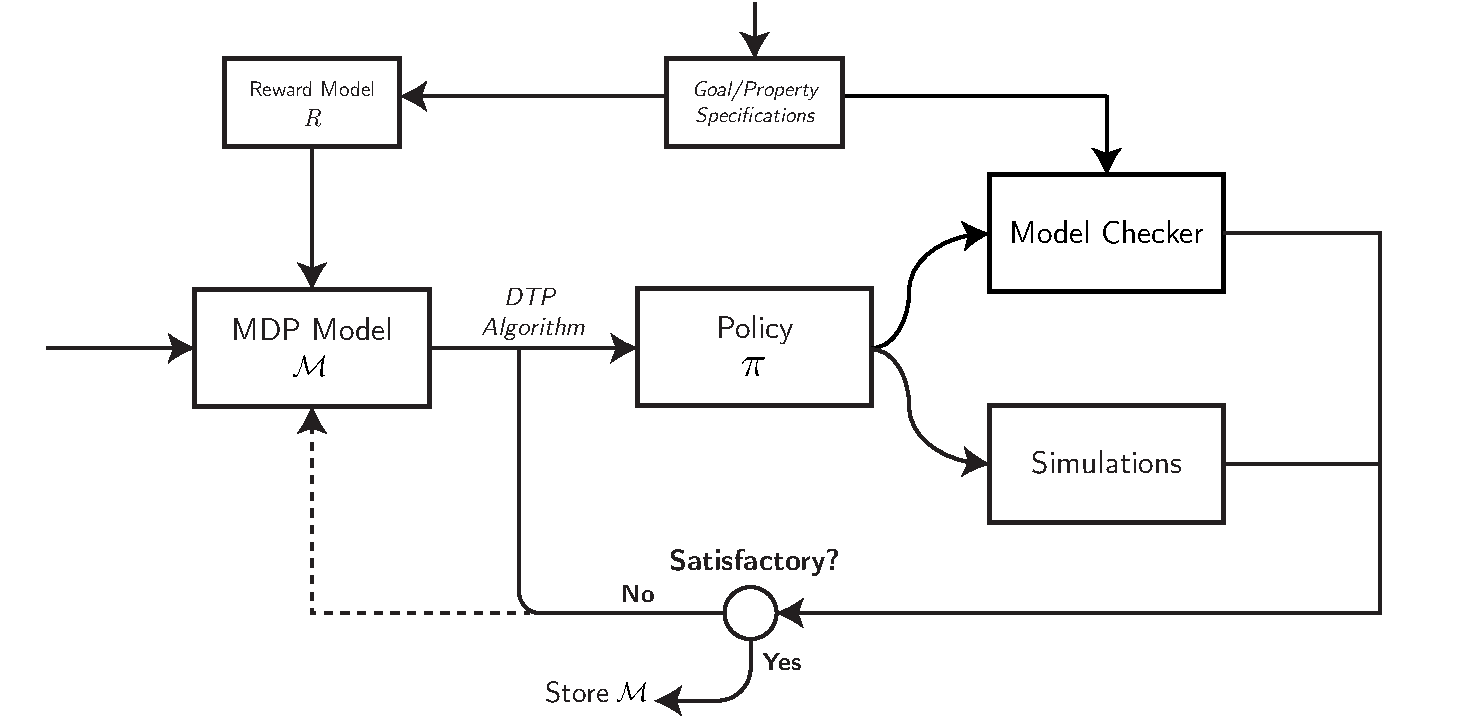
\includegraphics[width=0.9\textwidth]{figures/mdp-planning-diagram-v32-cropped}
\end{center}
\end{frame}

\begin{frame}
	\frametitle{Planning under Uncertainty}
	\framesubtitle{Model Development}
	
	\textcolor{tudBlack}{\textbf{Problem:}} How to obtain a suitable MDP for offline planning?
	\pause
	\vfill
	\textcolor{tudBlack}{\textbf{Classical approach:}} Model development by a \textit{human designer}, however:
	\begin{itemize}
		\item Requires significant effort (e.g., trial-and-error)
		\item Typically demands knowledge/experience, accompanied by high costs
	\end{itemize}
	\pause
	\vfill
	\textcolor{tudBlack}{\textbf{Alternative:}} Use Reinforcement Learning instead of Planning, however:
	\begin{itemize}
		\item Requires direct interaction with environment %(slow in complex dynamic environment) % (chance of errors)
		\item One might require \textit{reusable} models, applicable for multiple tasks % You do have model-based RL, but we might want a model that generalizes for multiple tasks
		%\item Still requires definition of state-spaces (and actions and rewards)
	\end{itemize}
\end{frame}

\begin{frame}[t]
	\frametitle{Planning under Uncertainty}
	\framesubtitle{Model Development}
	\vspace{8pt}
	\textcolor{tudBlack}{\textbf{Problem:}} How to obtain a suitable MDP for offline planning?\\
	\vspace{14pt}
	\textcolor{tudblue}{\textbf{Idea:}} Automate the model development process \\through learning algorithms 
	\begin{itemize}
		\item Learn from (exploration) data about the environment
		\item Optimization for the best MDP model
	\end{itemize}

\end{frame}

\begin{frame}
\frametitle{Problem Description}
\framesubtitle{Problem Statement}



\end{frame}

\begin{frame}
\frametitle{Problem Description}
\framesubtitle{Related Work}



\end{frame}

\begin{frame}
\frametitle{Problem Description}
\framesubtitle{Research Questions}

\begin{block}{Main Research Question}
%	How can the task of learning a \textit{performance-maximizing} MDP from a dataset be automated?
How can the task of obtaining an MDP that maximizes the yielded performance of executing plans that are derived from it, given a dataset about the system under consideration, be automated? %TODO Probably too long text, use shorter version?
\end{block}

\end{frame}